\section{Design}

Designing a user interface for such a game is not the simplest of endeavours because, unlike most games where the UI is
an afterthought, in Wisim the user interface is a make or break factor for the game. As with many simulation games where
the game acts as interface with which the player interacts with an underlying simulation like Hearts of Iron 4 or
OpenTTD, the interface has to turn the abstract parameters and numbers of the simulation into concrete, understandable
information that the player would understand in the context.

\subsection{Design Philosophy and Layout}

The most fundamental question in designing the game is which philosophy and layout to choose. Should I use a tabular
layout and simply lay the data out in an almost 1:1 connection to the simulation or should there be a sort of dashboard
representing what an executive might get on their desk or should the game's UI visually show the physical conditions of
an enterprise?

Answering this question is tough and took significant time, however there are some options that could be ruled out
quickly:

\begin{itemize}
	\item A physical representation of the enterprise that shows how machines, offices, etc would exist physically
	      \rightarrow Such a design would have a scope far outside of what is reasonable within half a year.

	\item A simple tabular layout that resembles how the data is represented in the back-end \rightarrow My judgment tells
	      me that a design like that would make the game rather boring and unintuitive. The values displayed would be too
	      abstracted from what they represent and would just lead to confusion.
\end{itemize}

\subsubsection{Attempt \#1: Tabular Dashboard}

The first attempt at a design was made in made in April 2025 with a tabular layout with hints of a more advanced
dashboard. It was very helpful for testing out various aspects of the simulation, however it proved simply too abstract
to be immersive all the while many operations were painfully slow and some mechanics could not reasonably be implemented
while following the existing designs (such as individual management of personnel and machines).

\begin{figure}[h]
	\centering
	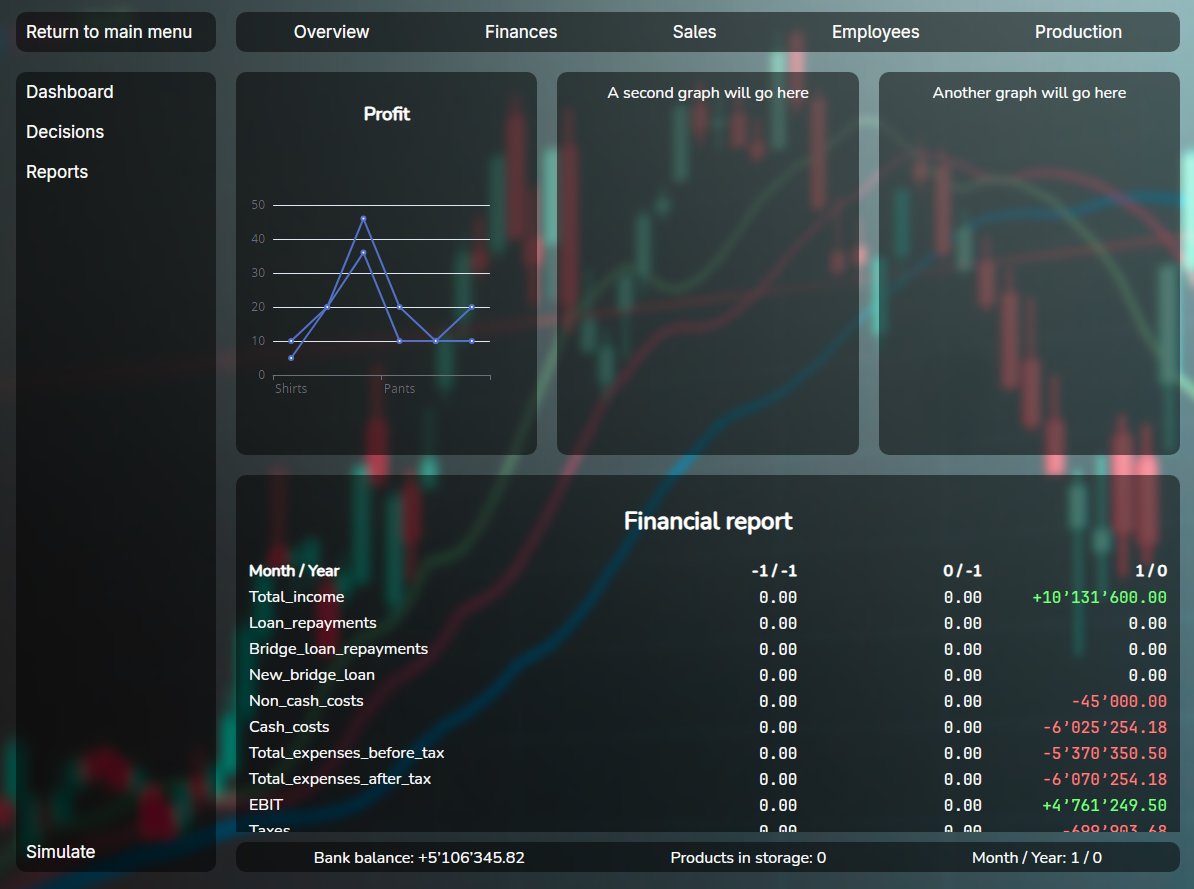
\includegraphics[width=0.45\textwidth]{wisimLayout1.png}
	\caption{The first UI I made for the game}
\end{figure}

\subsubsection{Attempt \#2: Desktop Management system}

\subsection{Product Designer}

One example: the product designer. In early versions of the game, the product designer was simply a menu of sliders, all
of which changed a certain stat in an unpredicatable and unrepeatable manner. This design was an unspectacular mix of
boring, unintuative and intimidating. During early playtesting players repeatedly asked what each slider did and
\textit{why} it did it. Understanding what was actually happening was tremendously difficult and theoretical (like
playing and Excel table).

\begin{figure}[h!]
	\centering
	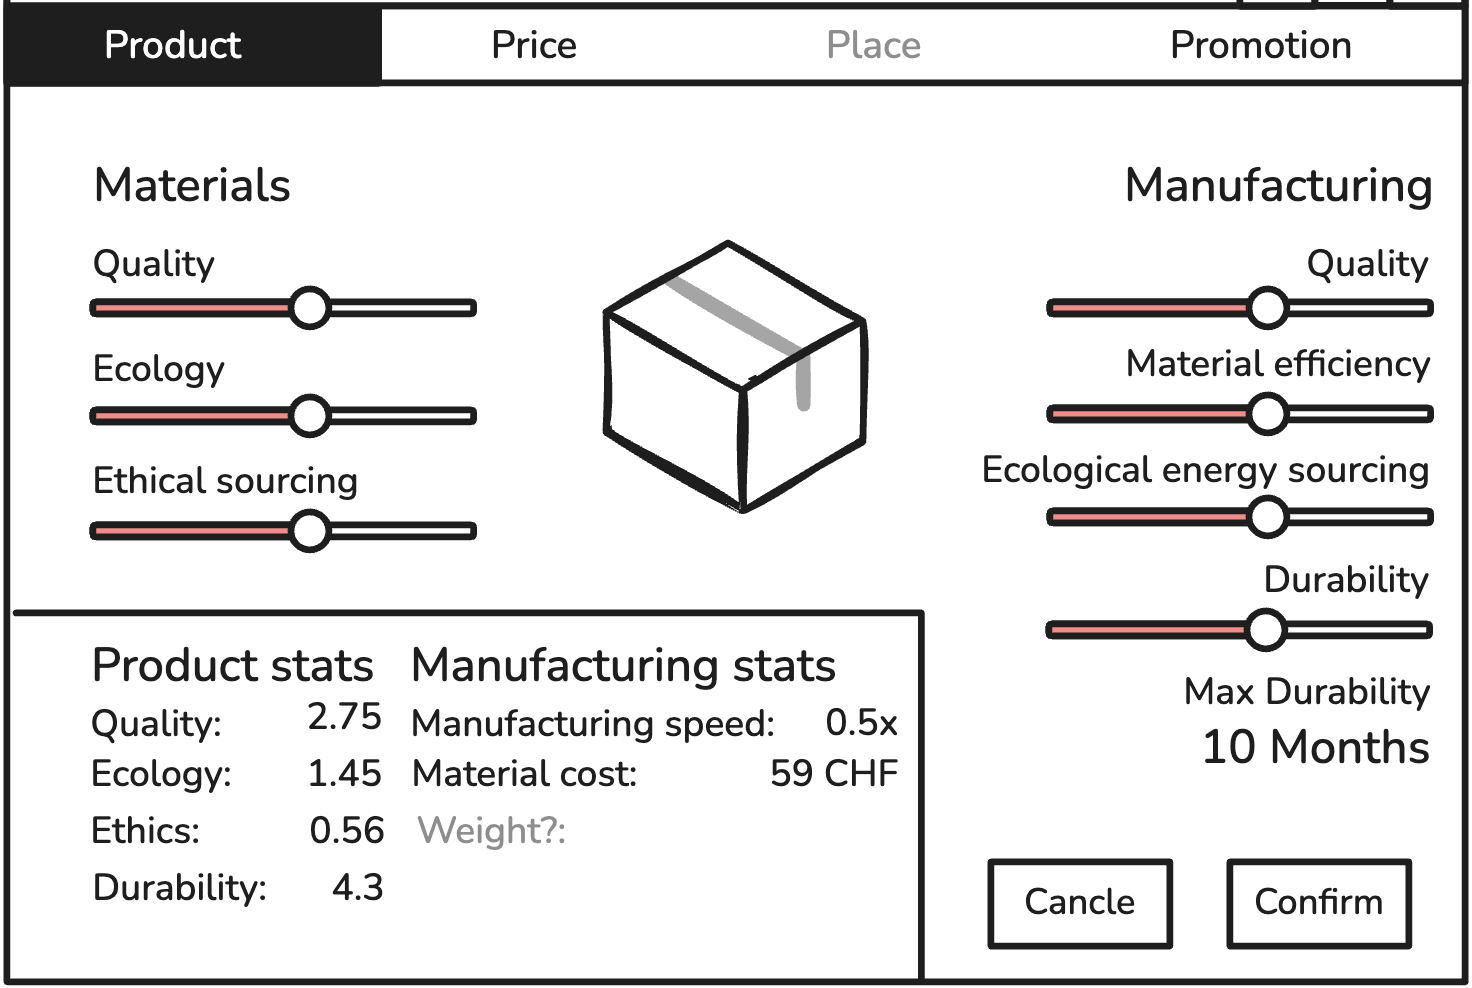
\includegraphics[width=0.45\textwidth]{product.png}
	\caption{The original product designer}
\end{figure}

\begin{figure}[h!]
	\centering
	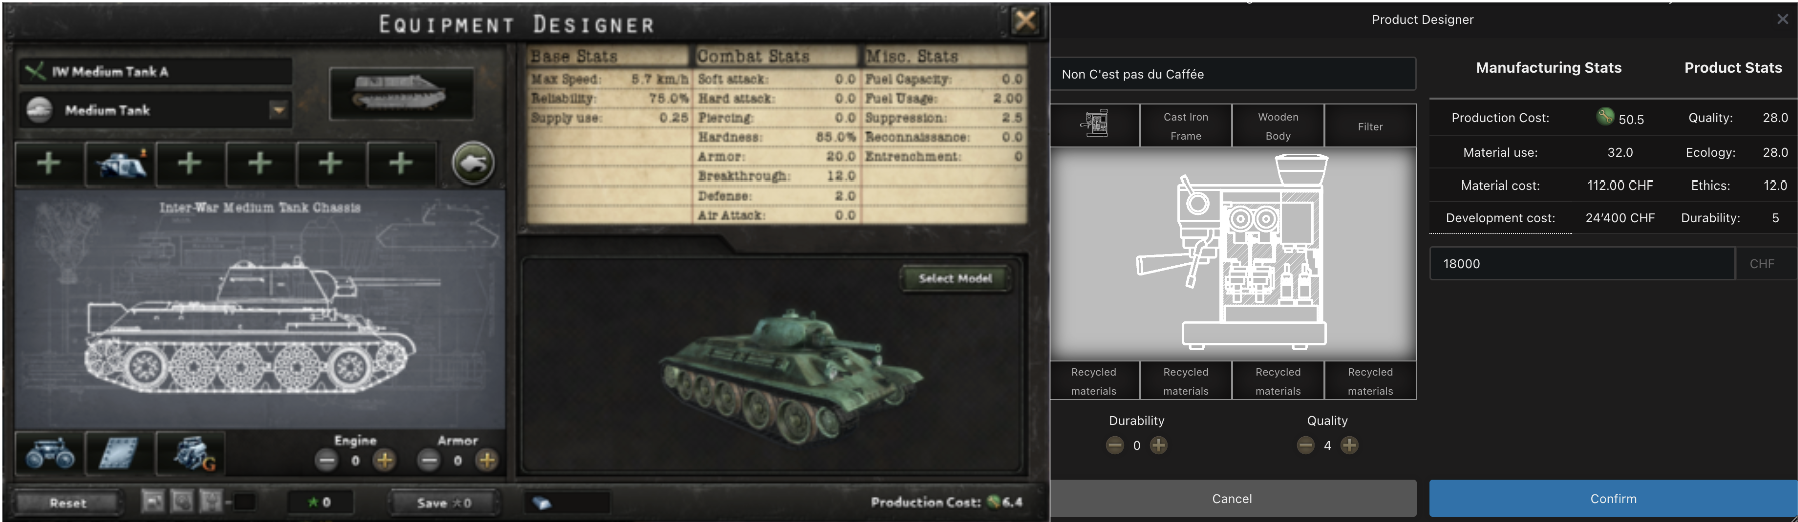
\includegraphics[width=0.85\textwidth]{product-designer-hoi4-wisim.png}
	\caption{The tank designer from Hearts of Iron 4 (left) and product designer from Wisim (right)}
\end{figure}

Thinking of how to fix the above problems, I remembered Hearts of Iron 4. Hearts of Iron is a WW2 simulation game and it
suffers from the same problem of making an Excel table fun to play. One of their early DLCs included a new tank designer
in which the player chose specific components to put in their tank. This system decreases the abstractness of the
content while still allowing for lots of creativity. Seeing the similarities between the 2 games I promptly adapted the
system to my game.

The product designer designer system did, however, require some major changes: the most important of which being that it needed a
concrete product to be produced. At this stage in the games development, each company was developing a generic
\textit{product}. And so after (very short) delibaration, I picked coffee machines, for no deeper reason than there was
a coffee machine sitting right in front of me.


